\chapter[Haar Measure and the p* Formula]{Right Haar Measure, Transformation Models and the p* Formula}\label{ch:11b}

In 1933 Alfr\'ed Haar proved that every separable locally compact group carries a measure invariant under translation \cite{haar1933}; von Neumann's uniqueness theorems and Weil's book of 1940 completed the theory in the generality used today. Statisticians met the same measure from the other side. Fisher's fiducial argument \cite{fisher1935}, Fraser's structural inference \cite{fraser1968} and the invariant estimation theory of Stein \cite{stein1965} and Hora and Buehler \cite{horabuehler1966} live on groups such as the affine group of the line, which are not unimodular: their left and right Haar measures differ, and the right one is the prior whose posterior reproduces the fiducial distribution and whose invariant credible sets have exact frequentist coverage. Barndorff Nielsen's $p^*$ formula \cite{barndorffnielsen1983} uses the left one: in a transformation model $|\hat\jmath|^{1/2}d\hat g$ is a left Haar measure, which is why $p^*$ is exact there.

This chapter puts the two traditions side by side, because the affine group of the line is, up to isomorphism, the triangular subgroup of $\SL_2(\R)$ that acts simply transitively on the upper half plane. Sato Tate groups are compact, so left and right Haar measures agree and Haar measure is the law of Frobenius (Chapter~\ref{ch:04}); in Chapter~\ref{ch:12} it enters the likelihood. The upper half plane, by contrast, is an orbit of a group that is not unimodular, and its hyperbolic area is the image of left Haar measure. Duke's theorem says that Heegner points equidistribute for this measure, a noncompact analogue of Sato Tate. Haar measures also normalise volumes, Tamagawa numbers and the period formulas behind central $L$ values. The statistical theorems are classical, and we prove Theorems~\ref{thm:11bpstar} and \ref{thm:11bright} in the generality of Definition~\ref{def:11bmodel}; Proposition~\ref{thm:11brefprior} on reference priors for conjugacy classes and the computations are new.

\section{Haar measure on locally compact groups}

Left and right Haar measures can differ. We define the modular function that measures the difference, compute both measures for the affine group and the Borel subgroup of $\GL_2$, and transport them to the upper half plane and the Bruhat Tits tree.

\subsection{Existence, uniqueness and the modular function}

Let $G$ be a locally compact Hausdorff group. A \emph{left Haar measure} is a nonzero Radon measure $\mu_l$ with $\mu_l(gE)=\mu_l(E)$ for all Borel $E$ and $g\in G$; a right Haar measure satisfies $\mu_r(Eg)=\mu_r(E)$.\index{Haar measure}

\begin{theorem}[Haar, von Neumann, Weil]\label{thm:11bhaar}
Every locally compact group has a left Haar measure, unique up to a positive constant.
\end{theorem}

Haar \cite{haar1933} proved existence for second countable groups; von Neumann proved uniqueness for compact groups \cite{vonneumann1934} and then for the groups of Haar's theorem \cite{vonneumann1936}; and Weil \cite{weil1940} proved existence and uniqueness without countability assumptions. A modern proof is in \cite{folland1995}. If $\mu_l$ is a left Haar measure and $g\in G$, then $E\mapsto\mu_l(Eg)$ is again left invariant, so by uniqueness
\begin{equation}\label{eq:11bmodular}
\mu_l(Eg)=\Delta_G(g)\,\mu_l(E)
\end{equation}
for a number $\Delta_G(g)>0$ independent of $E$. This is our convention for the \emph{modular function}; it is that of \cite{folland1995}. The map $\Delta_G:G\to\R_{>0}$ is a continuous homomorphism, and in differential form $d\mu_l(xg)=\Delta_G(g)\,d\mu_l(x)$.\index{modular function}

\begin{lemma}\label{thm:11bleftright}
The measure $d\mu_r(x)=\Delta_G(x)^{-1}d\mu_l(x)$ is a right Haar measure, and every right Haar measure is a multiple of it. For a Lie group $\Delta_G(g)=|\det\operatorname{Ad}(g)|^{-1}$.
\end{lemma}

\begin{proof}
Substituting $x=yg$ and using \eqref{eq:11bmodular},
\[\mu_r(Eg)=\int 1_{Eg}(x)\,\frac{d\mu_l(x)}{\Delta_G(x)}=\int 1_E(y)\,\frac{\Delta_G(g)\,d\mu_l(y)}{\Delta_G(y)\Delta_G(g)}=\mu_r(E).\]
Uniqueness follows from Theorem~\ref{thm:11bhaar} applied to the opposite group. For the Lie group formula, let $\mu_l$ be given by a left invariant volume form $\omega$, determined by its value $\omega_e$ on the Lie algebra. Right translation $R_g:x\mapsto xg$ commutes with left translations, so it pulls $\omega$ back to the left invariant form with value $\omega_e\circ\operatorname{Ad}(g^{-1})=\det\operatorname{Ad}(g)^{-1}\,\omega_e$ at $e$, and $\mu_l(Eg)=\int_E|R_g^*\omega|=|\det\operatorname{Ad}(g)|^{-1}\mu_l(E)$.
\end{proof}

$G$ is \emph{unimodular} if $\Delta_G\equiv1$, in which case left and right Haar measures coincide.\index{unimodular group}

\begin{example}[Unimodular groups]\label{ex:11bunimodular}
(i) Compact groups: $\Delta_G(G)$ is a compact subgroup of $\R_{>0}$, hence $\{1\}$. So a compact group, in particular a Sato Tate group, has exactly one Haar probability measure, and the phrase ``Haar measure'' in Chapters~\ref{ch:04} and \ref{ch:12} is unambiguous. (ii) $\GL_n(F)$ for $F=\R$ or $\Q_p$: on the matrix space $M_n(F)$ with additive Haar measure $dx$, left and right multiplication by $g$ both scale $dx$ by $|\det g|^n$, so $|\det x|^{-n}dx$ is a left and right Haar measure. (iii) $\SL_2(\R)$ and $\SL_2(\Q_p)$ are perfect groups, equal to their commutator subgroups, and $\Delta_G$ is a homomorphism into an abelian group, so it is trivial. (iv) Connected nilpotent Lie groups: every $g$ is $\exp X$ for some $X$ in the Lie algebra, and $\operatorname{Ad}(g)=\exp(\operatorname{ad}X)$ is unipotent, so $\det\operatorname{Ad}(g)=1$.
\end{example}

\subsection{The affine group and the Borel subgroup}

The simplest group that is not unimodular is the affine group of the line,
\[
B=\Bigl\{(a,b)=\begin{pmatrix}a&b\\0&1\end{pmatrix}:a>0,\ b\in\R\Bigr\},\qquad (a,b)(a',b')=(aa',ab'+b),
\]
acting on $\R$ by $x\mapsto ax+b$.\index{affine group}

\begin{proposition}\label{thm:11baffine}
On $B$, $d\mu_l=a^{-2}\,da\,db$ and $d\mu_r=a^{-1}\,da\,db$, and $\Delta_B(a,b)=a^{-1}$.
\end{proposition}

\begin{proof}
Left translation by $(\alpha,\beta)$ is the map $(a,b)\mapsto(\alpha a,\alpha b+\beta)$, whose Jacobian matrix with respect to $(a,b)$ is $\operatorname{diag}(\alpha,\alpha)$, of determinant $\alpha^2$. Hence for the image point $(a',b')$ we have $da'\,db'/a'^2=\alpha^2\,da\,db/(\alpha^2a^2)=da\,db/a^2$, so $a^{-2}da\,db$ is left invariant. Right translation by $(\alpha,\beta)$ is $(a,b)\mapsto(a\alpha,a\beta+b)$, with Jacobian matrix $\bigl(\begin{smallmatrix}\alpha&0\\\beta&1\end{smallmatrix}\bigr)$ of determinant $\alpha$; then $da'\,db'/a'=\alpha\,da\,db/(a\alpha)=da\,db/a$, so $a^{-1}da\,db$ is right invariant. Under the same right translation $da'\,db'/a'^2=\alpha^{-1}da\,db/a^2$, so $\Delta_B(\alpha,\beta)=\alpha^{-1}$ by \eqref{eq:11bmodular}, in agreement with $d\mu_r=\Delta_B^{-1}d\mu_l$.
\end{proof}

For the Borel subgroup $B_2=\{\bigl(\begin{smallmatrix}a&b\\0&d\end{smallmatrix}\bigr)\}$ of $\GL_2(F)$, $F=\R$ or $\Q_p$, the same Jacobian computation gives $d\mu_l=|a|^{-2}|d|^{-1}da\,db\,dd$, $d\mu_r=|a|^{-1}|d|^{-2}da\,db\,dd$ and $\Delta_{B_2}=|d/a|$ (Exercise~\ref{ex:11bborel}). The inverse $|a/d|$ is the character usually written $\delta_B$ in representation theory, and the normalised induction that defines principal series representations twists by $\delta_B^{1/2}$ precisely to compensate for the failure of unimodularity.

\subsection{Iwasawa decomposition}

Let $G=\SL_2(\R)$ with $K=\mathrm{SO}(2)$ and $B=B^+=\{n(x)a(y)\}$, where $n(x)=\bigl(\begin{smallmatrix}1&x\\0&1\end{smallmatrix}\bigr)$ and $a(y)=\operatorname{diag}(y^{1/2},y^{-1/2})$, $y>0$; or let $G=\GL_2(\Q_p)$ with $K=\GL_2(\Z_p)$ and $B$ the upper triangular group. In both cases $G=BK$ (Iwasawa decomposition), and a Haar measure $dg$ on the unimodular group $G$ factors through left Haar measure on $B$:\index{Iwasawa decomposition}
\begin{equation}\label{eq:11biwasawa}
\int_Gf(g)\,dg=\int_B\int_Kf(bk)\,d\mu_l(b)\,dk ,
\end{equation}
with $dk$ the Haar probability measure on $K$ \cite{bump1997,folland1995}. Formula \eqref{eq:11biwasawa} fixes the normalisation of $dg$; in the $p$ adic case, normalising $\mu_l$ so that the compact group $B\cap K$ has measure one gives $K$ measure one. The proof is the uniqueness argument again: $B\times K$ acts transitively on $G$ by $g\mapsto bgk^{-1}$ with compact stabiliser $B\cap K$, so a measure on $G$ invariant under this action is unique up to scale; Haar measure is one such measure because $G$ is unimodular, and the image of $\mu_l\times dk$ under $(b,k)\mapsto bk$ is another. It is the left, not the right, Haar measure of $B$ that appears.

\subsection{The upper half plane}

$\SL_2(\R)$ acts on $\mathbb H=\{x+iy:y>0\}$ by M\"obius transformations, the stabiliser of $i$ is $\mathrm{SO}(2)$, and so $\mathbb H=\SL_2(\R)/\mathrm{SO}(2)$. Since $n(x)a(y)\cdot z=yz+x$, the group $B^+$ is the affine group $(a,b)=(y,x)$ of Proposition~\ref{thm:11baffine}, acting on $\mathbb H$ simply transitively, and the orbit map $\phi(a,b)=(a,b)\cdot i=b+ia$ is a bijection $B^+\to\mathbb H$.

\begin{proposition}\label{thm:11bhyperbolic}
The image under $\phi$ of left Haar measure $a^{-2}da\,db$ is the hyperbolic area $dx\,dy/y^2$; the image of right Haar measure is $dx\,dy/y$. Every $B^+$ invariant Radon measure on $\mathbb H$ is a multiple of $dx\,dy/y^2$, and this measure is invariant under all of $\SL_2(\R)$. The measure $dx\,dy/y$ is not $B^+$ invariant.
\end{proposition}

\begin{proof}
In coordinates $\phi$ is $(a,b)\mapsto(x,y)=(b,a)$, so the images are as stated. Since $\phi(hg)=h\cdot\phi(g)$, a measure $m$ on $\mathbb H$ is $B^+$ invariant exactly when $\phi^{-1}_*m$ is left invariant on $B^+$; by Theorem~\ref{thm:11bhaar} these are the multiples of $a^{-2}da\,db$. For $g=\bigl(\begin{smallmatrix}\alpha&\beta\\\gamma&\delta\end{smallmatrix}\bigr)\in\SL_2(\R)$ the map $z\mapsto gz$ is holomorphic with derivative $(\gamma z+\delta)^{-2}$, so its real Jacobian is $|\gamma z+\delta|^{-4}$, while $\operatorname{Im}(gz)=y|\gamma z+\delta|^{-2}$; the two factors cancel in $dx\,dy/y^2$. Finally, for $c>0$ the measure $dx\,dy/y$ of $cE$ is $c$ times that of $E$.
\end{proof}

Thus hyperbolic area is the image of left Haar measure. The Iwasawa formula explains why it is invariant under the whole group although $B^+$ is not unimodular: on $G/K$ with $G$ unimodular and $K$ compact the invariant measure is the image of $dg$, and by \eqref{eq:11biwasawa} this image is the image of $d\mu_l$ on $B^+$.

\begin{figure}[t]
\centering
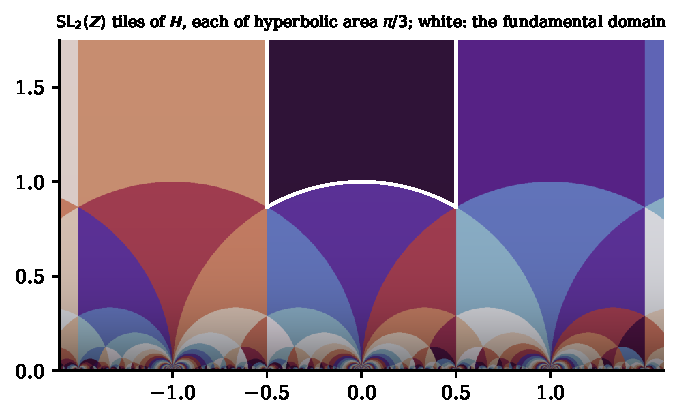
\includegraphics[width=\textwidth]{figs/modular_tessellation.pdf}
\caption{The tiles $\gamma\mathcal F$, $\gamma\in\SL_2(\Z)$, of the upper half plane, coloured by reduction depth; the standard fundamental domain $\mathcal F$ is outlined in white. Each tile has hyperbolic area $\pi/3$ for the left Haar image $dx\,dy/y^2$.}\label{fig:11btess}
\end{figure}

The standard fundamental domain of $\SL_2(\Z)$ is $\mathcal F=\{|x|\le\frac12,\ x^2+y^2\ge1\}$ (Figure~\ref{fig:11btess}), and its area is
\begin{equation}\label{eq:11barea}
\int_{-1/2}^{1/2}\int_{\sqrt{1-x^2}}^\infty\frac{dy}{y^2}\,dx=\int_{-1/2}^{1/2}\frac{dx}{\sqrt{1-x^2}}=2\arcsin\tfrac12=\frac\pi3 .
\end{equation}
Consequently $\frac3\pi\,dx\,dy/y^2$ is the invariant probability measure on $\SL_2(\Z)\backslash\mathbb H$. The Petersson inner product $\langle f,g\rangle=\int_{\mathcal F}f\bar g\,y^k\,dx\,dy/y^2$ of weight $k$ forms integrates against this measure, and Rankin and Selberg's unfolding, the source of $L(s,\Delta\times\Delta)$, uses the same invariance: with $\Gamma_\infty=\{\pm\bigl(\begin{smallmatrix}1&m\\0&1\end{smallmatrix}\bigr):m\in\Z\}$ and $E(z,s)=\sum_{\gamma\in\Gamma_\infty\backslash\SL_2(\Z)}\operatorname{Im}(\gamma z)^s$,
\[
\begin{split}\int_{\mathcal F}|\Delta(z)|^2y^{12}E(z,s)\,\frac{dx\,dy}{y^2}&=\int_0^\infty\!\!\int_0^1|\Delta|^2y^{s+10}\,dx\,dy\\&=\frac{\Gamma(s+11)}{(4\pi)^{s+11}}\sum_{n\ge1}\frac{\tau(n)^2}{n^{s+11}}\end{split}
\]
\cite{iwanieckowalski2004}. The Mellin integral $\Lambda(s,\Delta)=\int_0^\infty\Delta(iy)y^s\,dy/y$ of Chapter~\ref{ch:10} uses a third Haar measure, $dy/y$ on the diagonal torus, which is abelian and therefore unimodular.

\subsection{The Bruhat Tits tree and two Haar shadows}

For a prime $p$ the vertex set of the Bruhat Tits tree $\T_p$ of Chapter~\ref{ch:07} is
\[\GL_2(\Q_p)/\Q_p^\times\GL_2(\Z_p)=\PGL_2(\Q_p)/\PGL_2(\Z_p).\] Normalise Haar measure on the unimodular group $\PGL_2(\Q_p)$ so that the open compact subgroup $\PGL_2(\Z_p)$ has measure one. Each vertex is a coset $g\PGL_2(\Z_p)$, of measure one, so the image of Haar measure on the vertex set is counting measure, the unique invariant measure on a discrete homogeneous space up to scale.\index{Bruhat Tits tree}

Two probability measures on $[-2,2]$ come from Haar measures in this picture. The Plancherel measure of $\PGL_2(\Q_p)$ restricted to the unramified tempered dual, for this normalisation of Haar measure, is the Kesten McKay law $\mu_p$ (Macdonald \cite{macdonald1971}; Chapter~\ref{ch:07}). The Sato Tate law $\ST$ is the image of Haar measure on the compact group $\SU(2)$, the maximal compact subgroup of the dual group $\SL_2(\C)$, under the map to conjugacy classes. One is a shadow of Haar measure on a noncompact $p$ adic group, read through harmonic analysis; the other is a shadow of Haar measure on a compact real form of the complex dual group, read through Weyl's integration formula. They are related by the limit $\mu_p\Rightarrow\ST$ as $p\to\infty$ (Theorem~\ref{thm:07tree}), and arithmetically by Serre's vertical theorem (Theorem~\ref{thm:07serre}) against the horizontal Sato Tate theorem.

\section{Equidistribution on a noncompact quotient}\label{sec:11bduke}

The quotient $\SL_2(\Z)\backslash\mathbb H$ has finite volume but is not compact. Duke's theorem is the equidistribution theorem for its invariant probability measure $\frac3\pi\,dx\,dy/y^2$, the normalised image of left Haar measure.

\subsection{Duke's theorem}

Let $D<-4$ be a fundamental discriminant. A positive definite primitive binary quadratic form $Q=(a,b,c)$ with $b^2-4ac=D$ has a root $z_Q=(-b+i\sqrt{|D|})/(2a)$ in $\mathbb H$, and $Q$ is reduced exactly when $z_Q\in\mathcal F$ (with the usual boundary conventions). The set $\Lambda_D$ of these \emph{Heegner points} (also called CM points) has $h(D)$ elements, the class number of $\Q(\sqrt D)$ (Exercise~\ref{ex:11bclass}).\index{Heegner points}

\begin{theorem}[Duke \cite{duke1988}]\label{thm:11bduke}
As $D\to-\infty$ through fundamental discriminants, $\Lambda_D$ becomes equidistributed in $\SL_2(\Z)\backslash\mathbb H$ for $\frac3\pi\,dx\,dy/y^2$: for every Borel set $\Omega\subset\mathcal F$ whose boundary has measure zero,
\[
\frac{\#(\Lambda_D\cap\Omega)}{h(D)}\longrightarrow\frac3\pi\int_\Omega\frac{dx\,dy}{y^2}.
\]
\end{theorem}

We describe the proof only at the level of its inputs. By the Weyl criterion on the noncompact quotient one must show that the normalised Weyl sums $h(D)^{-1}\sum_{z\in\Lambda_D}\varphi(z)$ tend to $0$ for $\varphi$ a Maass cusp form and for the continuous spectrum. For the Eisenstein series the Weyl sum is an explicit multiple of $\zeta(s)L(s,\chi_D)$, and a subconvex bound for Dirichlet $L$ functions of Burgess type \cite{burgess1963} gives a power saving. For cusp forms Duke related the Weyl sums, through a theta correspondence, to Fourier coefficients of Maass forms of weight one half, and he bounded these coefficients by extending Iwaniec's method for holomorphic forms of half integral weight \cite{iwaniec1987}. Earlier, Linnik had proved the result under a congruence condition on $D$ by an ergodic method \cite{linnik1968}.

The Langlands content is visible through Waldspurger's theorem \cite{waldspurger1981}: the squares of the Fourier coefficients of a half integral weight form are proportional to the central values $L(\frac12,f\otimes\chi_D)$ of the quadratic twists of its Shimura lift $f$, and the toric period formula \cite{waldspurger1985} expresses $|\sum_{\Lambda_D}\varphi|^2$ through central values attached to $\varphi$ and to the quadratic field. In this language equidistribution follows from, and is essentially equivalent to, a subconvex bound for these central values in the $D$ aspect, and Iwaniec's estimate, extended by Duke to Maass forms, is such a bound. We do not attempt the exact constants, which depend on the Haar normalisations discussed in Section~\ref{sec:11btamagawa}.

\subsection{A computation}

For the $60$ fundamental discriminants $D$ in $[-1002999,-1002803]$ we enumerated all reduced primitive forms (computation for this book). There are $28251$ Heegner points, and for each $D$ the count equals the class number $h(D)$ returned by PARI/GP. Above height $t\ge1$ the fundamental domain is the strip $|x|\le\frac12$, so the invariant measure predicts
\[
\Prob(\operatorname{Im}z>t)=\frac3\pi\int_t^\infty\frac{dy}{y^2}=\frac3{\pi t},\qquad t\ge1,
\]
and, given $\operatorname{Im}z>1$, a uniform law for $\operatorname{Re}z$ on $[-\frac12,\frac12]$. Table~\ref{tab:11bduke} and Figure~\ref{fig:11bheegner} compare. The tail agrees with $3/(\pi t)$ to within $3\cdot10^{-3}$ at every height. In units of the binomial standard error $(P(1-P)/28251)^{1/2}$, $P=3/(\pi t)$, which is only a yardstick (the points are not random, and $z_Q$ and $-\bar z_Q$ have the same height), the deviation is $2.4$ at $t=1$ and below one at the other heights. Duke's proof gives a rate $|D|^{-\delta}$, and at $|D|\approx10^6$ this is at least $0.03$ for every $\delta\le\frac14$ (the Lindel\"of value, Computational Problem~\ref{cp:11bduke}), at least ten times the largest deviation. The table is therefore consistent with the theorem but does not test its rate. The horizontal coordinate above height one passes a Kolmogorov Smirnov test for uniformity with $p=0.36$.

\begin{table}[t]
\centering
\small\setlength{\tabcolsep}{4pt}
\begin{tabular}{lcccccc}
\toprule
$t$ & $1$ & $1.5$ & $2$ & $3$ & $5$ & $10$\\
\midrule
data & $0.95193$ & $0.63608$ & $0.47524$ & $0.31769$ & $0.19104$ & $0.09511$\\
$3/(\pi t)$ & $0.95493$ & $0.63662$ & $0.47746$ & $0.31831$ & $0.19099$ & $0.09549$\\
\bottomrule
\end{tabular}
\caption{Heights of the $28251$ Heegner points for the $60$ fundamental discriminants in $[-1002999,-1002803]$ against the invariant tail $3/(\pi t)$; the row ``data'' is the empirical $\Prob(\operatorname{Im}z>t)$.}\label{tab:11bduke}
\end{table}

\begin{figure}[t]
\centering
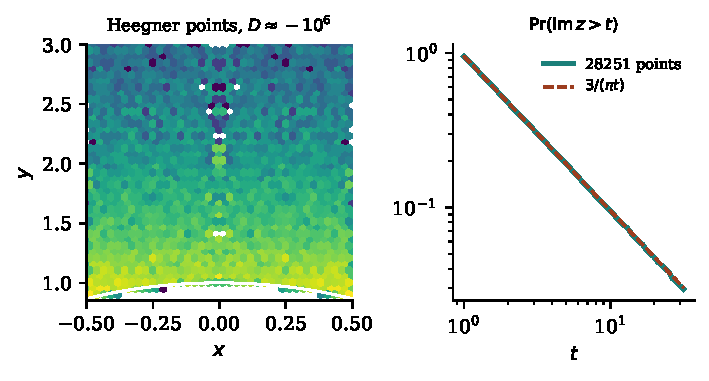
\includegraphics[width=\textwidth]{figs/haar_heegner.pdf}
\caption{Left: density of the $28251$ Heegner points of Table~\ref{tab:11bduke} in the fundamental domain, in hexagonal bins up to height $3$; lighter cells hold more points, and the density decays like $y^{-2}$. Right: the empirical tail $\Prob(\operatorname{Im}z>t)$ against the left Haar prediction $3/(\pi t)$ on logarithmic axes.}\label{fig:11bheegner}
\end{figure}

\begin{remark}[A noncompact Sato Tate theorem]
Sato Tate says that the classes of Frobenius equidistribute for Haar measure on a compact group. Duke's theorem says that the CM points of discriminant $D$ equidistribute for the invariant measure on $\SL_2(\Z)\backslash\SL_2(\R)/\mathrm{SO}(2)$, which on the Iwasawa coordinates is left Haar measure of $B^+$. In both, the limit law is a Haar measure and the proof needs an automorphic input, potential automorphy of symmetric powers \cite{blght2011} in one case and subconvexity for twisted central values in the other. The difference is the cusp: mass could escape to $y=\infty$, and the convergence of $\Prob(\operatorname{Im}z>t)$ to $3/(\pi t)$, which tends to $0$ as $t\to\infty$, says that it does not.
\end{remark}

\section{Transformation models and the p* formula}

In a transformation model the conditional law of the maximum likelihood estimator given an ancillary configuration is explicit, and Barndorff Nielsen's $p^*$ formula reproduces it exactly; outside such models $p^*$ is an approximation of high order.

\subsection{Structural models}

Following Fraser \cite{fraser1968} and Barndorff Nielsen \cite{barndorffnielsen1983,barndorffnielsencox1994}, a \emph{transformation model} is a family of laws generated from one law by a group. We work in the following setting.\index{transformation model}

\begin{definition}\label{def:11bmodel}
Let $G$ be a Lie group of dimension $d$ acting freely on an open set $\mathcal X\subset\R^n$ by affine maps $x\mapsto A_gx+b_g$, and put $\chi(g)=|\det A_g|$, a continuous homomorphism $G\to\R_{>0}$. Let $U$ have a density $f$ on $\mathcal X$, twice continuously differentiable on the open set where it is positive. The \emph{transformation model} is the family of laws of $X=gU$, $g\in G$, with densities
\[
p(x;g)=f(g^{-1}x)\,\chi(g)^{-1}.
\]
We assume that for every $x$ in an open $G$ invariant set $\mathcal X_0\subset\mathcal X$ of full measure the likelihood $g\mapsto p(x;g)$ has a unique maximiser $\hat g(x)$, that $\hat g$ is smooth on $\mathcal X_0$, and that the observed information $j(\hat g;x)=-\nabla^2\ell(\hat g)$, $\ell(g)=\log p(x;g)$, is nonsingular in some (hence every) chart.
\end{definition}

The location scale model $X_i=\mu+\sigma U_i$, $n\ge2$, is the case $G=B$, $g=(\sigma,\mu)$, $\chi(g)=\sigma^n$, with $\mathcal X=\{x\in\R^n:\text{not all }x_i\text{ equal}\}$, on which $B$ acts freely; the scale model $X_i=\theta U_i$ on $(0,\infty)^n$ is the case $G=\R_{>0}$.

\begin{lemma}\label{thm:11bconfig}
(i) $\hat g(hx)=h\hat g(x)$ for $h\in G$. (ii) The \emph{configuration} $a(x)=\hat g(x)^{-1}x$ is a maximal invariant, so its law does not depend on $g$: it is ancillary. (iii) $x=\hat g(x)\,a(x)$, and $A=\{x\in\mathcal X_0:\hat g(x)=e\}$ is a smooth submanifold of dimension $n-d$ such that $\Phi:G\times A\to\mathcal X_0$, $\Phi(h,a)=ha$, is a diffeomorphism.
\end{lemma}

\begin{proof}
(i) $p(hx;g)=f(g^{-1}hx)\chi(g)^{-1}=p(x;h^{-1}g)\chi(h)^{-1}$, so $g$ maximises the left side if and only if $h^{-1}g$ maximises $p(x;\cdot)$, that is $g=h\hat g(x)$. (ii) $a(hx)=\hat g(x)^{-1}h^{-1}hx=a(x)$; and if $a(x)=a(y)$ then $y=\hat g(y)\hat g(x)^{-1}x$ lies on the orbit of $x$. Since $X=gU$, $a(X)=a(U)$ has the law of $a(U)$ for every $g$. (iii) By (i) the derivative of $\hat g$ along the orbit through $x$ is onto, so $\hat g$ is a submersion and $A=\hat g^{-1}(e)$ is a submanifold; $\Phi$ is smooth with smooth inverse $x\mapsto(\hat g(x),\hat g(x)^{-1}x)$.
\end{proof}

\begin{lemma}\label{thm:11bdisint}
Under $\Phi$, Lebesgue measure on $\mathcal X_0$ becomes $\chi(h)\,d\mu_l(h)\,\kappa(da)$ for a measure $\kappa$ on $A$ with a smooth positive density.
\end{lemma}

\begin{proof}
The pull back $\nu(F)=\lambda(\Phi(F))$ of Lebesgue measure $\lambda$ under the diffeomorphism $\Phi$ has a smooth positive density, $\nu=q(h,a)\,d\mu_l(h)\,da$ with $da$ a smooth volume on $A$. Since $\Phi(g'h,a)=g'\Phi(h,a)$ and $\lambda(g'E)=\chi(g')\lambda(E)$, the measure $\nu$ satisfies $\nu(L_{g'}F)=\chi(g')\nu(F)$ for $L_{g'}(h,a)=(g'h,a)$. As $\mu_l$ is left invariant this says $q(g'h,a)=\chi(g')q(h,a)$, hence $q(h,a)=\chi(h)q(e,a)$. Put $\kappa(da)=q(e,a)\,da$.
\end{proof}

\subsection{Exactness of p*}

Barndorff Nielsen's formula approximates the conditional density of the maximum likelihood estimator given an ancillary $a$ by\index{p* formula}
\begin{equation}\label{eq:11bpstar}
p^*(\hat g;g\mid a)=c(a)\,|j(\hat g;x)|^{1/2}\exp\{\ell(g)-\ell(\hat g)\},
\end{equation}
where $x$ is reconstructed from $(\hat g,a)$, $\ell$ is the log likelihood, the density is taken with respect to Lebesgue measure in a chart of $G$, and $c(a)$ makes it integrate to one.

\begin{theorem}[Barndorff Nielsen \cite{barndorffnielsen1980,barndorffnielsen1983}]\label{thm:11bpstar}
In the transformation model of Definition~\ref{def:11bmodel}, conditionally on the maximal invariant $a(X)=a$, the estimator $\hat g$ has density
\begin{equation}\label{eq:11bexact}
p(\hat g;g\mid a)=\frac{f(g^{-1}\hat g\,a)\,\chi(g^{-1}\hat g)}{c_0(a)}\qquad\text{with respect to }d\mu_l(\hat g),
\end{equation}
$c_0(a)=\int_Gf(ka)\chi(k)\,d\mu_l(k)$. Moreover $|j(\hat g;x)|^{1/2}d\hat g=|j(e;a)|^{1/2}\,d\mu_l(\hat g)$ in any chart, with $\mu_l$ normalised to agree with chart Lebesgue measure at $e$, and \eqref{eq:11bpstar} is exactly \eqref{eq:11bexact}.
\end{theorem}

For the location scale group the exact conditional density is due to Fisher \cite{fisher1934}; the identification with $p^*$, and the point that $|\hat\jmath|^{1/2}d\hat g$ is left invariant, are Barndorff Nielsen's. The proof below is written for the generality of Definition~\ref{def:11bmodel}.

\begin{proof}
By Lemma~\ref{thm:11bdisint} the joint density of $(\hat g,a)=\Phi^{-1}(X)$ with respect to $d\mu_l(h)\,\kappa(da)$ is $p(ha;g)\chi(h)=f(g^{-1}ha)\chi(g^{-1}h)$. Dividing by its integral over $h$ gives \eqref{eq:11bexact}, and $c_0(a)<\infty$ for $\kappa$ almost every $a$ by Fubini, since the joint density integrates to one.

For the information, fix $x=\hat g a$ and write $\ell_x(g)=\log p(x;g)$. From $p(\hat ga;g)=f(g^{-1}\hat ga)\chi(g)^{-1}$ we get $\ell_x(g)=\ell_a(\hat g^{-1}g)-\log\chi(\hat g)$. In a chart let $\psi$ denote $g\mapsto\hat g^{-1}g$. Since $e$ maximises $\ell_a$ (because $\hat g(a)=e$), its gradient vanishes there, so the chain rule gives no first order term and
\[
j(\hat g;x)=D\psi(\hat g)^{\top}\,j(e;a)\,D\psi(\hat g),\qquad |j(\hat g;x)|^{1/2}=|\det D\psi(\hat g)|\,|j(e;a)|^{1/2}.
\]
A left invariant measure has chart density $m(g)=m(e)|\det D(L_{g^{-1}})(g)|$, which is $|\det D\psi(\hat g)|$ at $g=\hat g$ when $m(e)=1$. This proves the second claim. Finally
\[
\exp\{\ell_x(g)-\ell_x(\hat g)\}=\frac{f(g^{-1}\hat ga)\chi(g)^{-1}}{f(a)\chi(\hat g)^{-1}}=\frac{f(g^{-1}\hat ga)\chi(g^{-1}\hat g)}{f(a)},
\]
so $p^*\,d\hat g=c(a)|j(e;a)|^{1/2}f(a)^{-1}f(g^{-1}\hat ga)\chi(g^{-1}\hat g)\,d\mu_l(\hat g)$, which is \eqref{eq:11bexact} for $c(a)=f(a)/(c_0(a)|j(e;a)|^{1/2})$.
\end{proof}

\begin{example}[Location and scale]\label{ex:11blocscale}
For $X_i=\mu+\sigma U_i$ with $\hat g=(\hat\sigma,\hat\mu)$, the configuration is $a=(a_i)$ with $a_i=(x_i-\hat\mu)/\hat\sigma$, $\chi(g)=\sigma^n$, and by Proposition~\ref{thm:11baffine} $d\mu_l=d\hat\mu\,d\hat\sigma/\hat\sigma^2$. With $f$ now the density of each $U_i$, Theorem~\ref{thm:11bpstar} gives the conditional density of $(\hat\mu,\hat\sigma)$ given $a$ as proportional to $\hat\sigma^{n-2}\sigma^{-n}\prod_if((\hat\mu-\mu+\hat\sigma a_i)/\sigma)$, Fisher's formula. Directly, $j(\hat g;x)=\hat\sigma^{-2}H(a)$ with $H(a)$ a function of the configuration alone, so $|\hat\jmath|^{1/2}=\hat\sigma^{-2}|H(a)|^{1/2}$ is the left Haar density.
\end{example}

\begin{example}[Exponential scale family]\label{ex:11bexp}
Let $X_1,\dots,X_n$ be independent with density $\theta^{-1}e^{-x/\theta}$ on $(0,\infty)$. Then $\ell(\theta)=-n\log\theta-n\bar x/\theta$, $\hat\theta=\bar x$, $\ell(\hat\theta)=-n\log\hat\theta-n$, and $\ell''(\theta)=n\theta^{-2}-2n\bar x\theta^{-3}$, so $j(\hat\theta)=n/\hat\theta^2$. Hence
\[
p^*(\hat\theta;\theta)=c\,\frac{n^{1/2}}{\hat\theta}\,\frac{\hat\theta^n e^n}{\theta^n}\,e^{-n\hat\theta/\theta}=c\,n^{1/2}e^n\,\frac{\hat\theta^{n-1}}{\theta^n}\,e^{-n\hat\theta/\theta}.
\]
The exact law of $\bar X$ is Gamma with shape $n$ and rate $n/\theta$, with density
\[p(\hat\theta;\theta)=\frac{(n/\theta)^n\hat\theta^{n-1}e^{-n\hat\theta/\theta}}{\Gamma(n)},\]
the same function of $\hat\theta$, so after normalisation, $c=n^{n-1/2}e^{-n}/\Gamma(n)$, $p^*$ is exact. (The configuration $x/\bar x$ is independent of $\bar x$ here, so conditioning is vacuous.) With the unnormalised constant $c=(2\pi)^{-1/2}$ the ratio $p^*/p$ is $\Gamma(n)e^n/(\sqrt{2\pi}\,n^{n-1/2})=1+\frac1{12n}+O(n^{-2})$ by Stirling's formula; numerically $1.0168$, $1.0084$, $1.0042$ for $n=5,10,20$.
\end{example}

\subsection{Beyond group models}

Outside transformation models $p^*$ is an approximation. For a full exponential family and $n$ independent observations, $\hat\theta$ is sufficient, no ancillary is needed, and $p^*$ coincides with the saddlepoint approximation of Daniels \cite{daniels1954} to the density of the sufficient statistic, transformed to $\hat\theta$. With $c=(2\pi)^{-d/2}$ its relative error is $O(n^{-1})$. After renormalisation the relative error is $O(n^{-3/2})$ on normal deviation regions, where $\hat\theta-\theta=O(n^{-1/2})$, and remains $O(n^{-1})$ for larger deviations \cite{barndorffnielsen1983,barndorffnielsencox1994,reid1988}. In curved exponential families the order $O(n^{-3/2})$ holds conditionally on an ancillary that is exact or approximately ancillary to sufficiently high order \cite{barndorffnielsen1980,barndorffnielsencox1994}. Laplace's method explains the shape: expanding $\ell(\theta)-\ell(\hat\theta)$ to second order around $\hat\theta$ makes \eqref{eq:11bpstar} with $c=(2\pi)^{-d/2}$ approximately a normal density for $\hat\theta$ with mean $\theta$ and covariance $\hat\jmath^{-1}$, and $(2\pi)^{-d/2}|\hat\jmath|^{1/2}$ is its normalising constant. Example~\ref{ex:11bexp} shows two of these levels: the constant $(2\pi)^{-1/2}$ is off by Stirling's factor $1+\frac1{12n}+O(n^{-2})$, while the renormalised formula is exact because the model is a group model.

\section{Right Haar priors}\label{sec:11bright}

We prove that the right Haar prior gives invariant credible sets exact frequentist coverage, compute the shortfall of the left Haar prior for normal errors, and check both by simulation.

\subsection{Structural, fiducial and Bayes}

The posterior of the right Haar prior coincides with Fraser's structural distribution and with Fisher's fiducial distribution, and its invariant credible sets are exact confidence sets for every sample size \cite{fraser1968,stein1965,horabuehler1966}; see also \cite{berger1985,eaton1989}. We give a complete proof in the setting of Definition~\ref{def:11bmodel}.\index{right Haar prior}

\begin{theorem}[Fraser; Stein; Hora and Buehler]\label{thm:11bright}
Let the prior be $d\mu_r(g)$, and let $x\in\mathcal X_0$ have configuration $a$ with $c_0(a)<\infty$, which holds for almost every $x$. Under the posterior, the pivot $k=g^{-1}\hat g(x)$ has law
\[
Q_a(dk)=c_0(a)^{-1}f(ka)\chi(k)\,d\mu_l(k),
\]
and under the sampling law $P_g$, conditionally on $a(X)=a$, the pivot $g^{-1}\hat g(X)$ has the same law $Q_a$. Consequently, if $S_a\subset G$ satisfies $Q_a(S_a)=1-\alpha$ for each $a$, the set $C(x)=\{g:g^{-1}\hat g(x)\in S_{a(x)}\}$ has posterior probability $1-\alpha$ and $P_g(g\in C(X))=1-\alpha$ for every $g\in G$ and every $n$.
\end{theorem}

\begin{proof}
The posterior is proportional to $p(x;g)\,d\mu_r(g)$. Inversion carries $\mu_r$ to a left Haar measure, and by \eqref{eq:11bmodular} right translation by $\hat g$ multiplies left Haar measure by a constant; so the image of $\mu_r$ under $g\mapsto k=g^{-1}\hat g$ is a constant multiple of $\mu_l$. With $g=\hat gk^{-1}$ and $x=\hat ga$,
\[
p(x;\hat gk^{-1})=f(k\hat g^{-1}\hat ga)\,\chi(\hat gk^{-1})^{-1}=f(ka)\chi(k)\chi(\hat g)^{-1},
\]
and $\chi(\hat g)$ is constant given $x$. So the posterior of $k$ is $Q_a$, a proper law because $c_0(a)<\infty$. Under $P_g$, Theorem~\ref{thm:11bpstar} gives the conditional density $f(g^{-1}\hat ga)\chi(g^{-1}\hat g)/c_0(a)$ of $\hat g$ with respect to $d\mu_l(\hat g)$, and $k=g^{-1}\hat g$ is a left translate of $\hat g$, so its density with respect to $d\mu_l(k)$ is $f(ka)\chi(k)/c_0(a)$. The coverage statement follows by conditioning on $a$ and then averaging over it.
\end{proof}

The proof uses only the equivariance $\hat g(hx)=h\hat g(x)$ and the decompositions of Lemmas~\ref{thm:11bconfig}(iii) and \ref{thm:11bdisint}, and these hold for any smooth equivariant map $\mathcal X_0\to G$ in place of $\hat g$. So Theorem~\ref{thm:11bright} needs neither a unique maximum likelihood estimator nor any smoothness of $f$: in the location scale model the pair $(s,\bar x)$, with $s$ the sample standard deviation, serves on all of $\mathcal X$.

\begin{corollary}\label{thm:11bcoverage}
In the location scale model with prior $d\mu\,d\sigma/\sigma$, the equal tailed $1-\alpha$ posterior intervals for $\mu$ and for $\sigma$ have frequentist coverage exactly $1-\alpha$ for every $n\ge2$ and every error density $f$.
\end{corollary}

\begin{proof}
Let $\hat g=(\hat\sigma,\hat\mu)$ be $(s,\bar x)$, which by the remark above is allowed for every $f$, and write $k=g^{-1}\hat g=(\rho,\tau)$ with $\rho=\hat\sigma/\sigma$ and $\tau=(\hat\mu-\mu)/\sigma$. Then $(\mu-\hat\mu)/\hat\sigma=-\tau/\rho$ and $\sigma/\hat\sigma=1/\rho$ are functions of $k$ alone. The posterior quantiles of $\mu$ are $\hat\mu+\hat\sigma q_\pm(a)$ with $q_\pm(a)$ the quantiles of $-\tau/\rho$ under $Q_a$, so the event that the interval covers $\mu$ is $\{-\tau/\rho\in[q_-(a),q_+(a)]\}$, of the form in Theorem~\ref{thm:11bright}. The same argument applies to $\sigma$.
\end{proof}

\subsection{Left Haar priors}

Jeffreys' rule gives $d\mu\,d\sigma/\sigma^2$ for location and scale \cite{jeffreys1961}, the left Haar measure. Since $d\mu_l=\Delta_G\,d\mu_r$, the same computation shows that under the left Haar prior the pivot has law proportional to $\Delta_G(\hat gk^{-1})Q_a(dk)\propto\Delta_G(k)^{-1}Q_a(dk)$, a tilt of $Q_a$. For location and scale $\Delta_G(k)^{-1}=\rho$, so the tilt favours large $\hat\sigma/\sigma$, that is small $\sigma$: intervals for $\mu$ are too short, those for $\sigma$ sit too low, and in the examples below coverage falls below nominal. For normal errors this is explicit (our calculation): the left Haar posterior of $\mu$ is a $t$ law with $n$ rather than $n-1$ degrees of freedom, centre $\bar x$ and scale $S^{1/2}/n$, $S=\sum(x_i-\bar x)^2$, and that of $S/\sigma^2$ is $\chi^2_n$ rather than $\chi^2_{n-1}$. Writing $t_{\nu,q}$ and $\chi^2_{\nu,q}$ for $q$ quantiles and $T_\nu$, $\chi^2_\nu$ for random variables with these laws, the exact coverages of the $90\%$ equal tailed intervals at $n=5$ are $\Prob(|T_4|\le t_{5,0.95}\sqrt{4/5})=0.854$ for $\mu$ and $\Prob(\chi^2_{5,0.05}\le\chi^2_4\le\chi^2_{5,0.95})=0.861$ for $\sigma$.

\subsection{A computation with the P\'olya variable of $\Delta$}

As error law we take the P\'olya variable $W$ of Chapter~\ref{ch:10}, with density $\Phi_\Delta(u)\propto\Delta(ie^u)e^{6u}$: symmetric, with doubly exponential tails much lighter than Gaussian ones. With $n=5$, true $(\mu,\sigma)=(1.3,0.7)$ and $4000$ replications, we computed $90\%$ equal tailed posterior intervals on a grid centred and scaled by each data set, so that the computation is itself equivariant (computation for this book). Table~\ref{tab:11bcoverage} and Figure~\ref{fig:11bposterior} report the result. The right Haar coverages $0.9005$ and $0.898$ are within one Monte Carlo standard error ($0.0047$) of $0.9$, as Corollary~\ref{thm:11bcoverage} predicts; the left Haar coverages $0.860$ and $0.865$ are $8.4$ and $7.4$ standard errors short. For normal errors ($1000$ replications, standard error about $0.01$) the coverages are $0.909$, $0.908$ (right) and $0.869$, $0.870$ (left), against the exact values $0.9$ and $0.854$, $0.861$.

\begin{table}[t]
\centering
\begin{tabular}{lcccc}
\toprule
 & \multicolumn{2}{c}{P\'olya variable of $\Delta$} & \multicolumn{2}{c}{normal}\\
prior & $\mu$ & $\sigma$ & $\mu$ & $\sigma$\\
\midrule
right Haar $d\mu\,d\sigma/\sigma$ & $0.9005$ & $0.898$ & $0.909$ & $0.908$\\
left Haar $d\mu\,d\sigma/\sigma^2$ & $0.860$ & $0.865$ & $0.869$ & $0.870$\\
\bottomrule
\end{tabular}
\caption{Coverage of $90\%$ equal tailed posterior intervals, $n=5$; $4000$ replications for the P\'olya shape (standard error $0.0047$), $1000$ for the normal shape.}\label{tab:11bcoverage}
\end{table}

\begin{figure}[t]
\centering
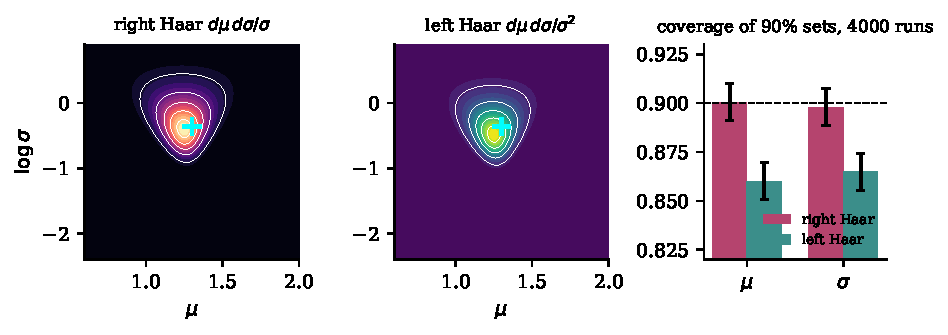
\includegraphics[width=\textwidth]{figs/haar_posterior.pdf}
\caption{Left and centre: right and left Haar posterior densities of $(\mu,\log\sigma)$ for one data set of size $5$ with P\'olya errors; the cross marks the true value $(1.3,\log0.7)$. Right: coverage of $90\%$ equal tailed intervals for $\mu$ and $\sigma$ over $4000$ replications, with bars of two Monte Carlo standard errors; the dashed line is the nominal level.}\label{fig:11bposterior}
\end{figure}

\subsection{Matching and paradoxes}

Theorem~\ref{thm:11bright} makes the right Haar prior an \emph{exact} probability matching prior for $\mu$ and for $\sigma$, stronger than the first order matching of Welch and Peers \cite{welchpeers1963}. Exactness needs only the free action. Optimality needs more: for an invariant loss the Bayes procedure of the right Haar prior is the best equivariant procedure \cite{horabuehler1966,eaton1989}, and by the Hunt Stein theorem the best equivariant procedure is minimax when $G$ is amenable, as the solvable group $B$ is; for the general linear group acting on covariance matrices, which is not amenable, Stein showed that it need not be \cite{eatongeorge2021}.

Dawid, Stone and Zidek \cite{dawidstonezidek1973} showed that improper priors can produce marginalisation paradoxes, in which the posterior of a parameter $\theta$ depends on the data only through a statistic $z$ whose law depends only on $\theta$, and yet no prior on $\theta$ reproduces it from the likelihood of $z$. In group models the paradox is avoided when the prior is right Haar measure on the group that leaves $\theta$ invariant, times any prior on $\theta$. Exercise~\ref{ex:11bparadox} works the classical case $\theta=\mu/\sigma$: here the relevant group is the scale group, the prior free of paradox is $d\mu\,d\sigma/\sigma^2$, and the right Haar prior $d\mu\,d\sigma/\sigma$ of the location scale group produces the paradox. ``Right'' is relative to the group that leaves the parameter of interest invariant; this is the starting point of Chang and Eaves.

\section{Reference priors for orbits}

When the parameter of interest is an orbit of a group acting on the parameter space, reference priors combine Haar measure on the group with a prior on the space of orbits. Conjugacy classes, and hence Satake parameters, are orbits of this kind.

\subsection{Chang and Eaves}

Let $G$ act freely on a parameter space, and let the parameter of interest be the orbit, equivalently a maximal invariant $\theta$. Chang and Eaves \cite{changeaves1990} showed that the prior combining right Haar measure on $G$ with a limiting form of Jeffreys' prior for the maximal invariant coincides with Bernardo's reference prior \cite{bernardo1979,bergerbernardo1992} when the orbit is the parameter of interest. Their prior can be computed without a product parametrisation, and their examples include the correlation matrix and the eigenvalues of a covariance matrix. For a one dimensional maximal invariant, Datta and J. K. Ghosh \cite{dattaghosh1995} compared reference, Chang Eaves and probability matching priors, judged them by marginalisation paradoxes and by frequentist matching, and concluded that the Chang Eaves and Berger Bernardo reference priors are the most attractive; Datta and M. Ghosh \cite{dattaghosh1996} studied which noninformative priors are invariant under reparametrisation.\index{reference prior}

\subsection{Conjugacy classes as orbits}

The Satake parameter of an unramified local representation is a conjugacy class in the dual group, an orbit of the adjoint action; when the representation is tempered it is a class in a compact group $K$, such as a Sato Tate group. We propose (this book) the following model for inference on such a class from noisy group elements. Let $K$ be a compact connected Lie group with Haar probability measure $dh$, let $\varphi\ge0$ be a smooth class function with $\int\varphi\,dh=1$, and observe $Y_1,\dots,Y_n$ independent with density
\begin{equation}\label{eq:11bnoise}
p(y\mid M)=\varphi(M^{-1}y)\quad\text{with respect to }dh,\qquad M=\eta\,t\,\eta^{-1},
\end{equation}
that is $Y=M\varepsilon$ with $\varepsilon$ of density $\varphi$. Examples are the heat kernel $\varphi_s=\sum_\rho\dim\rho\,e^{-sc_\rho}\chi_\rho$ ($c_\rho$ the Casimir eigenvalue) and, for $K=\SU(2)$, the von Mises Fisher law $\varphi(\varepsilon)\propto\exp(\kappa\operatorname{Re}\tr\varepsilon)$. The parameter of interest is the class of $M$, coordinatised by $t$ in a Weyl chamber $T^+$ of a maximal torus $T$; the nuisance parameter is $u=\eta T\in K/T$. Conjugation is not free on $K$, so the theorem of Chang and Eaves does not apply as stated. We instead compute the reference prior directly, with the two group algorithm of Berger and Bernardo \cite{bergerbernardo1992}, ordered as (class, conjugator): on a compact parameter space with information matrix $I=\bigl(\begin{smallmatrix}I_{11}&I_{12}\\I_{21}&I_{22}\end{smallmatrix}\bigr)$,
\begin{equation}\label{eq:11bbb}
\pi(u\mid t)\propto|I_{22}(t,u)|^{1/2},\qquad \pi(t)\propto\exp\Bigl\{\int\pi(u\mid t)\log|I_{11\cdot2}(t,u)|^{1/2}\,du\Bigr\},
\end{equation}
with $I_{11\cdot2}=I_{11}-I_{12}I_{22}^{-1}I_{21}$.

\begin{proposition}[this book]\label{thm:11brefprior}
Let $K$ be compact, connected and simple, and suppose the Fisher information of \eqref{eq:11bnoise} at $M=e$ is finite and nonsingular. Then:
\begin{enumerate}
\item[(i)] The Fisher metric is $c\,n$ times a fixed bi invariant Riemannian metric on $K$, for a constant $c=c(\varphi)>0$; Jeffreys' prior for $M$ is Haar measure, and its image on classes has the Weyl density $|W|^{-1}\prod_{\alpha}|e^{i\alpha(t)}-1|$ (product over all roots) with respect to the Haar probability measure $dt$ of $T$: it is the Sato Tate measure of $K$.
\item[(ii)] The reference prior \eqref{eq:11bbb} is the product of the $K$ invariant probability measure on $K/T$ and the uniform (Haar) measure $dt$ on the Weyl chamber. Its image on classes is the image of Haar measure on the torus $T$.
\end{enumerate}
For $K=\SU(2)$ the reference prior for the angle $\theta\in[0,\pi]$ is $d\theta/\pi$, so $x=2\cos\theta$ has the arcsine law, against the Sato Tate prior $\frac2\pi\sin^2\theta\,d\theta$. For $K=\USp(4)$ it is uniform on $0\le\theta_2\le\theta_1\le\pi$, against the density proportional to $(\cos\theta_1-\cos\theta_2)^2\sin^2\theta_1\sin^2\theta_2$ of Proposition~\ref{thm:12usp4}.
\end{proposition}

\begin{proof}
(i) The group $K\times K$ acts on parameters and data by $(g_1,g_2)\cdot M=g_1Mg_2^{-1}$, $(g_1,g_2)\cdot y=g_1yg_2^{-1}$, preserving $dh$, and $p(g_1yg_2^{-1}\mid g_1Mg_2^{-1})=\varphi(g_2M^{-1}yg_2^{-1})=\varphi(M^{-1}y)$ because $\varphi$ is a class function. So the Fisher metric is invariant under left and right translations. At $e$ it is an $\operatorname{Ad}(K)$ invariant inner product on the Lie algebra $\mathfrak k$, and since $K$ is simple $\operatorname{Ad}$ is irreducible, so by Schur's lemma the inner product is a multiple $c$ of a fixed invariant one; $c>0$ by the nonsingularity assumption, and independence multiplies it by $n$. The Riemannian volume of a bi invariant metric is Haar measure, and the image on classes is given by Weyl's integration formula.

(ii) On the regular set write $M=\eta t\eta^{-1}$ with $t$ in the interior of the Weyl chamber; since the centraliser of a regular $t$ is $T$, the map $(\eta T,t)\mapsto M$ is a diffeomorphism onto the regular set, whose complement has Haar measure zero. For $Y\in\mathfrak t$ the tangent vector $\frac{d}{ds}\eta te^{sY}\eta^{-1}$ is the left translate by $\eta t\eta^{-1}$ of $\operatorname{Ad}(\eta)Y$; for $X\in\mathfrak t^\perp$, $\frac{d}{ds}\eta e^{sX}te^{-sX}\eta^{-1}$ is the left translate of $\operatorname{Ad}(\eta)(\operatorname{Ad}(t^{-1})X-X)$. The bi invariant metric is $\operatorname{Ad}$ invariant, $\mathfrak t^\perp$ is $\operatorname{Ad}(t)$ stable, so torus and orbit directions are orthogonal: $I_{12}=0$ and $I_{11\cdot2}=I_{11}=cn\,\|\cdot\|^2_{\mathfrak t}$, constant in $(t,u)$. On a root plane $\mathfrak k_\alpha\subset\mathfrak t^\perp$, $\operatorname{Ad}(t^{-1})$ is a rotation by the angle $\alpha(t)$, so $\|\operatorname{Ad}(t^{-1})X-X\|=|e^{i\alpha(t)}-1|\,\|X\|$, and therefore $|I_{22}(t,u)|^{1/2}=(cn)^{\dim K/T/2}\prod_{\alpha>0}|e^{i\alpha(t)}-1|^2\,v(u)$, with $v$ the density of the invariant volume of $K/T$. In \eqref{eq:11bbb}, normalising over $u\in K/T$ removes the factor depending on $t$, so $\pi(u\mid t)$ is the invariant probability on $K/T$; and $I_{11\cdot2}$ is constant, so $\pi(t)$ is uniform. The image of $dt$ on $T^+=T/W$ is the image of Haar measure on $T$. For $\SU(2)$ the chamber is $\theta\in[0,\pi]$, and for $\USp(4)$, $W$ is generated by sign changes and the swap, with chamber $0\le\theta_2\le\theta_1\le\pi$.
\end{proof}

Proposition~\ref{thm:11brefprior} splits Weyl's formula into two parts. The Vandermonde factor $\prod_\alpha|e^{i\alpha}-1|$ is the volume of the conjugacy orbit, nuisance information about the conjugator, and the reference prior removes it. The result agrees with the formal Chang Eaves recipe: Haar measure on the conjugating group times Jeffreys' prior for $t$ with $\eta$ known, which is uniform because $I_{11}$ is constant. The two priors on classes of $\SU(2)$ are far apart: by Lemma~\ref{thm:12integral},
\[
\mathrm{KL}\Bigl(\frac{d\theta}{\pi}\Big\|\frac2\pi\sin^2\theta\,d\theta\Bigr)=\log2,\qquad\mathrm{KL}\Bigl(\frac2\pi\sin^2\theta\,d\theta\Big\|\frac{d\theta}{\pi}\Bigr)=1-\log2,
\]
using $\int_0^\pi\log\sin\theta\,d\theta=-\pi\log2$. The reference prior is the normalised continuous part of the law $\mu_{\mathrm{CM}}$ of Chapter~\ref{ch:04}: the reference prior for a class of $\SU(2)$ is the Sato Tate law of the torus. Which prior to use depends on the question. For the class of a single Frobenius element of a curve without complex multiplication, the Sato Tate law is the correct prior. For the class of an unknown group element observed through isotropic noise, with no arithmetic information, the reference prior is uniform on the torus. Anisotropic noise, or an unknown noise level, breaks the block structure and is left as Computational Problem~\ref{cp:11bchangeaves}.

\section{Haar measure behind L values}\label{sec:11btamagawa}

Haar measures normalise the volumes in special value formulas; we record three instances without proofs.\index{Tamagawa number}

\emph{Volumes and zeta values.} With $dx\,dy/y^2$, $\operatorname{vol}(\SL_2(\Z)\backslash\mathbb H)=\pi/3=2\zeta(2)/\pi$ by \eqref{eq:11barea}. More generally, with Haar measure on $\SL_n(\R)$ normalised through Lebesgue measure on matrices, $\operatorname{vol}(\SL_n(\Z)\backslash\SL_n(\R))=\zeta(2)\zeta(3)\cdots\zeta(n)$; this goes back to Minkowski and was proved by Siegel \cite{siegel1945}, whose analytic theory of quadratic forms, including the average measure of \cite{siegel1944}, led to the Siegel Weil formula.

\emph{Tamagawa numbers.} For a semisimple group $H$ over $\Q$, an invariant differential form of top degree defines Haar measures on every $H(\Q_v)$; their product is a measure on $H(\A)$ independent of the form by the product formula, and $\tau(H)=\operatorname{vol}(H(\Q)\backslash H(\A))$. Weil proved $\tau(\SL_2)=1$ \cite{weil1961}. The mechanism is visible in a sketch. Strong approximation gives
\[
\SL_2(\Q)\backslash\SL_2(\A)=\SL_2(\Z)\backslash\Bigl(\SL_2(\R)\times\prod_p\SL_2(\Z_p)\Bigr),
\]
so $\tau(\SL_2)$ is the product of the archimedean volume $\operatorname{vol}(\SL_2(\Z)\backslash\SL_2(\R))=\zeta(2)$ and the volumes $\#\SL_2(\mathbb F_p)/p^3=1-p^{-2}$ of the groups $\SL_2(\Z_p)$, all for the form measure; since $\prod_p(1-p^{-2})=\zeta(2)^{-1}$, the product is $1$.

\emph{Period formulas.} Waldspurger's formula \cite{waldspurger1985} expresses the square of a toric period of a $\GL_2$ automorphic form, for example a Weyl sum over Heegner points, as a central value $L(\frac12,\pi_K)$ divided by $L(1,\pi,\operatorname{Ad})$, times local factors. Ichino and Ikeda \cite{ichinoikeda2010} formulated the analogue for $\mathrm{SO}(n+1)\times\mathrm{SO}(n)$ periods, as a refinement of the Gross Prasad conjecture, and verified it in low rank cases. In both, the global constant is fixed only once Tamagawa measures are chosen on the groups and their subgroups, and each local factor is an integral of matrix coefficients against local Haar measure. The Duke computation of Section~\ref{sec:11bduke} is the case where all these normalisations are hidden in $\frac3\pi$.

\section{Notes}

The Iwasawa integration formula and the half plane are treated in \cite{bump1997}. Fisher's conditional argument for location and scale is \cite{fisher1934} and his fiducial argument \cite{fisher1935}; structural inference is Fraser's \cite{fraser1968}. The $p^*$ formula, its exactness for transformation models and its accuracy elsewhere are due to Barndorff Nielsen \cite{barndorffnielsen1980,barndorffnielsen1983}, with the systematic treatment in \cite{barndorffnielsencox1994} and the survey \cite{reid1988}; the saddlepoint method is Daniels' \cite{daniels1954}. Stein \cite{stein1965} and Hora and Buehler \cite{horabuehler1966} identified Bayes procedures under right Haar priors with best invariant procedures and fiducial distributions; Eaton's lectures \cite{eaton1989} give the general theory of group invariance in statistics and Berger \cite{berger1985} the decision theoretic setting; Eaton and George \cite{eatongeorge2021} trace Stein's work on invariance from the Hunt Stein theorem to his counterexamples for groups that are not amenable. Marginalisation paradoxes are from \cite{dawidstonezidek1973}; reference priors from \cite{bernardo1979,bergerbernardo1992}, and for orbits from Chang and Eaves \cite{changeaves1990}, compared by Datta and J. K. Ghosh \cite{dattaghosh1995}; Datta and M. Ghosh \cite{dattaghosh1996} treat their invariance. Duke's theorem is \cite{duke1988}, building on Iwaniec \cite{iwaniec1987}, with Waldspurger's formulas \cite{waldspurger1981,waldspurger1985} giving the $L$ function interpretation; Linnik's ergodic method is in \cite{linnik1968}. Proposition~\ref{thm:11bhyperbolic} and Theorems~\ref{thm:11bpstar} and \ref{thm:11bright} are classical; only the proofs of the two theorems in the generality of Definition~\ref{def:11bmodel} are written for this book. Ours are Proposition~\ref{thm:11brefprior}, the exact normal coverages of Section~\ref{sec:11bright} and the computations, all elementary consequences of the cited theory.

\section{Exercises}

\begin{enumerate}
\item Verify Proposition~\ref{thm:11baffine} through Lemma~\ref{thm:11bleftright}: compute $\operatorname{Ad}(a,b)$ on the Lie algebra of $B$ in the basis $\bigl(\begin{smallmatrix}1&0\\0&0\end{smallmatrix}\bigr)$, $\bigl(\begin{smallmatrix}0&1\\0&0\end{smallmatrix}\bigr)$, and check $\Delta_B=|\det\operatorname{Ad}|^{-1}=a^{-1}$. Show that no nonzero Radon measure on $\R$ is invariant under all the maps $x\mapsto ax+b$, although $B$ acts transitively on $\R$.
\item\label{ex:11bborel} For the Borel subgroup of $\GL_2(F)$, $F=\R$ or $\Q_p$, prove that
\[d\mu_l=|a|^{-2}|d|^{-1}da\,db\,dd,\qquad d\mu_r=|a|^{-1}|d|^{-2}da\,db\,dd\]
and $\Delta_{B_2}=|d/a|$. Check that $\Delta_{B_2}$ is trivial on the unipotent radical and on the centre.
\item Show that for the normal location scale model $p^*$ is exact without conditioning, by computing $j(\hat\mu,\hat\sigma)=\operatorname{diag}(n,2n)/\hat\sigma^2$ and comparing \eqref{eq:11bpstar} with the joint density of $\bar X$ and $\hat\sigma^2=S/n$, using independence and $S/\sigma^2\sim\chi^2_{n-1}$. Identify the constant $c$.
\item Compute the hyperbolic area of the fundamental domain of $\Gamma_0(2)$ by showing that it is the union of $[\SL_2(\Z):\Gamma_0(2)]=3$ translates of $\mathcal F$, and of $\Gamma_0(p)$ in general. Derive \eqref{eq:11barea} also from the Gauss Bonnet formula for the triangle with angles $\pi/3$, $\pi/3$, $0$.
\item\label{ex:11bclass} Let $D<-4$ be a fundamental discriminant. Show that $Q\mapsto z_Q$ is injective, that $\SL_2(\Z)$ equivalence of forms corresponds to the action on roots, and that each class of primitive positive definite forms of discriminant $D$ contains exactly one reduced form; deduce that $\#\Lambda_D=h(D)$. Show that $\operatorname{Im}z_Q=\sqrt{|D|}/(2a)$, so that $\operatorname{Im}z_Q>t$ if and only if $a<\sqrt{|D|}/(2t)$, and use this to compute the tail counts of Table~\ref{tab:11bduke} from the list of reduced forms.
\item\label{ex:11bparadox} (Marginalisation paradox.) Let $X_1,\dots,X_n$ be independent $N(\mu,\sigma^2)$, $\theta=\mu/\sigma$, $T=\sum X_i^2$, $U=\sum X_i$, $z=U/\sqrt T$, and take the prior $\sigma^{-r}d\mu\,d\sigma$. Show that the posterior of $\theta$ is proportional to
\[e^{-n\theta^2/2}\int_0^\infty v^{n+r-3}e^{-v^2/2+\theta zv}dv,\]
which depends on the data only through $z$, and that the law of $z$ has density proportional to $(1-z^2/n)^{(n-3)/2}e^{-n\theta^2/2}\int_0^\infty v^{n-1}e^{-v^2/2+\theta zv}dv$. Conclude that a prior $\pi(\theta)$ reproduces the first posterior from the law of $z$ if and only if $r=2$, and observe that $d\mu\,d\sigma/\sigma^2=d\theta\,d\sigma/\sigma$ is Lebesgue measure in $\theta$ times the Haar measure $d\sigma/\sigma$ of the scale group $x\mapsto cx$, $c>0$, which leaves $\theta$ and $z$ invariant.
\end{enumerate}

\section{Open computational problems}

\begin{compproblem}[Duke rates at large discriminant]\label{cp:11bduke}
Objective: measure the rate in Theorem~\ref{thm:11bduke}. Objects: Heegner points for all fundamental discriminants with $|D|\le10^9$, and for samples of discriminants near $10^{10}$, $10^{11}$ and $10^{12}$ (class numbers up to about $10^6$). Route: enumerate reduced forms with PARI/GP \texttt{qfbred} and \texttt{qfbclassno} on a cluster, or generate the class group from prime forms with GPU batch reduction. Deliverable: the discrepancy of $\Lambda_D$ against $\frac3\pi dx\,dy/y^2$ over hyperbolic disks and over the tail sets $\operatorname{Im}z>t$, and the Weyl sums of the first ten Maass cusp forms (from the LMFDB), with fitted exponents $\delta$ in $|D|^{-\delta}$. Why it matters: Waldspurger's formula turns the Weyl sums into central $L$ values, so the fitted exponents test the subconvexity input and the Lindel\"of prediction $\delta=\frac14$ for the cusp form sums.
\end{compproblem}

\begin{compproblem}[Reference priors for anisotropic noise]\label{cp:11bchangeaves}
Objective: extend Proposition~\ref{thm:11brefprior} beyond bi invariant noise. Objects: $\SU(2)$ and $\USp(4)$ with matrix Fisher noise $\varphi(\varepsilon)\propto\exp(\operatorname{Re}\tr(F\varepsilon))$ for nonscalar $F$, and the heat kernel $\varphi_s$ with the time $s$ unknown. Route: Fisher information by Weyl integration and Gauss quadrature on the torus, then the Berger Bernardo algorithm with the class first, and the Chang Eaves recipe with right Haar measure on the stabiliser free part. Deliverable: the reference prior on classes as a density on the Weyl chamber, its Kullback Leibler distance to the Weyl density and to the torus Haar measure, and frequentist coverage of reference posterior sets for the class at $n=5,20,100$. Why it matters: it decides whether the Vandermonde factor of the Sato Tate measure survives in objective inference on Satake parameters when the noise is not symmetric.
\end{compproblem}

\begin{compproblem}[p* and right Haar intervals for angular models]\label{cp:11bpstar}
Objective: measure what the group structure buys for $p^*$ and for Haar priors in models built from Sato Tate data. Objects: the location and scale models $x_i=\mu+\sigma\varepsilon_i$ with $\varepsilon_i$ distributed by $\ST$, by the $\USp(4)$ trace law and by $\Phi_\Delta$; the von Mises model on the circle with unknown rotation, a group model, and with unknown rotation and concentration, a full exponential family that is not a group model; $n$ from $5$ to $200$. Route: exact conditional densities and constants $c(a)$ from Theorem~\ref{thm:11bpstar} by quadrature over the group, exact and saddlepoint densities for the two parameter von Mises model, and $10^5$ replications per setting in vectorised code. Deliverable: tables of the ratio $(2\pi)^{-d/2}/c(a)$ of unnormalised $p^*$ to the exact conditional density, as a function of $n$ and of the configuration; of the relative error of renormalised $p^*$ in the two parameter von Mises model; and of the coverage of right and left Haar intervals. Why it matters: in the group models renormalised $p^*$ and right Haar intervals are exact whatever the error law (Theorems~\ref{thm:11bpstar} and \ref{thm:11bright}), but the accuracy of the unnormalised formula rests on Laplace's method. The $\USp(4)$ trace density vanishes to fourth order at $\pm4$ and $\Phi_\Delta$ is smooth, so those models are regular, while the semicircle vanishes like a square root at $\pm2$ and has infinite Fisher information for location; the tables show whether the $O(n^{-1})$ accuracy of the constant survives in this nonregular model, and how the exact group answers compare with the $O(n^{-3/2})$ approximation outside group models.
\end{compproblem}

\begin{compproblem}[CM points and Hecke orbits on Shimura curves]\label{cp:11bshimura}
Objective: test equidistribution for Haar measure on compact quotients of $\mathbb H$. Objects: the Shimura curves attached to the maximal orders of the quaternion algebras over $\Q$ of discriminant $6$, $10$ and $14$; CM points of discriminant $|D|\le10^8$, and Hecke orbits $T_{p^k}x$ for the primes $p\le7$ not dividing the discriminant and $p^k\le10^7$. Route: Magma or Sage quaternion arithmetic for optimal embeddings, explicit fundamental domains (Voight's algorithms) for the hyperbolic coordinates. Deliverable: discrepancy against the normalised hyperbolic area, the decay rate in $|D|$ and in $p^k$, and for Hecke orbits a comparison with the rate $(k+1)p^{-k/2}$ that the Ramanujan conjecture for the Maass forms of the curve predicts (the random walk generated by $T_p$ has the corresponding Kesten rate $(2\sqrt p/(p+1))^k$ of Chapter~\ref{ch:07}). Why it matters: there is no cusp here, so the noncompact effects of Table~\ref{tab:11bduke} disappear; Hecke orbits are images of the Bruhat Tits tree of $\PGL_2(\Q_p)$ in the curve, which joins Chapter~\ref{ch:07} to the invariant measure of this chapter, and their decay rate is a numerical test of the Ramanujan conjecture for Maass forms, which is open.
\end{compproblem}
